
%(BEGIN_QUESTION)
% Copyright 2006, Tony R. Kuphaldt, released under the Creative Commons Attribution License (v 1.0)
% This means you may do almost anything with this work of mine, so long as you give me proper credit

Design en termistorkrets som gir en økende utgangsspenning når temperaturen øker.  Hint: topologien kan være så enkel som dette:

$$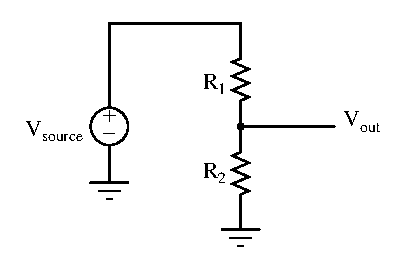
\includegraphics[width=15.5cm]{i00042x01.eps}$$

Du må velge hvilken motstand ($R_1$ eller $R_2$) som skal være termistor og hvilken som skal være fast, og også velge hvilken temperaturkoeffisient termistoren skal ha (enten {\it positiv} eller {\it negativ}).  Etter at du har gjort disse valgene og tegnet kretsen nedenfor, forklar hvordan den fungerer (dvs. hva som skjer med alle spenninger og strømmer når temperaturen øker):

\vfil 

\underbar{file i00042}
\eject
%(END_QUESTION)





%(BEGIN_ANSWER)

Dette er et vurdert spørsmål -- ingen svar eller hint gis!

%(END_ANSWER)





%(BEGIN_NOTES)

Enten gjør $R_1$ til termistor med {\it negativ} temperaturkoeffisient, eller gjør $R_2$ til termistor med {\it positiv} temperaturkoeffisient.

%INDEX% Measurement, temperature: thermistor circuit

%(END_NOTES)
